\documentclass[1p]{elsarticle_modified}
%\bibliographystyle{elsarticle-num}

%\usepackage[colorlinks]{hyperref}
%\usepackage{abbrmath_seonhwa} %\Abb, \Ascr, \Acal ,\Abf, \Afrak
\usepackage{amsfonts}
\usepackage{amssymb}
\usepackage{amsmath}
\usepackage{amsthm}
\usepackage{scalefnt}
\usepackage{amsbsy}
\usepackage{kotex}
\usepackage{caption}
\usepackage{subfig}
\usepackage{color}
\usepackage{graphicx}
\usepackage{xcolor} %% white, black, red, green, blue, cyan, magenta, yellow
\usepackage{float}
\usepackage{setspace}
\usepackage{hyperref}

\usepackage{tikz}
\usetikzlibrary{arrows}

\usepackage{multirow}
\usepackage{array} % fixed length table
\usepackage{hhline}

%%%%%%%%%%%%%%%%%%%%%
\makeatletter
\renewcommand*\env@matrix[1][\arraystretch]{%
	\edef\arraystretch{#1}%
	\hskip -\arraycolsep
	\let\@ifnextchar\new@ifnextchar
	\array{*\c@MaxMatrixCols c}}
\makeatother %https://tex.stackexchange.com/questions/14071/how-can-i-increase-the-line-spacing-in-a-matrix
%%%%%%%%%%%%%%%

\usepackage[normalem]{ulem}

\newcommand{\msout}[1]{\ifmmode\text{\sout{\ensuremath{#1}}}\else\sout{#1}\fi}
%SOURCE: \msout is \stkout macro in https://tex.stackexchange.com/questions/20609/strikeout-in-math-mode

\newcommand{\cancel}[1]{
	\ifmmode
	{\color{red}\msout{#1}}
	\else
	{\color{red}\sout{#1}}
	\fi
}

\newcommand{\add}[1]{
	{\color{blue}\uwave{#1}}
}

\newcommand{\replace}[2]{
	\ifmmode
	{\color{red}\msout{#1}}{\color{blue}\uwave{#2}}
	\else
	{\color{red}\sout{#1}}{\color{blue}\uwave{#2}}
	\fi
}

\newcommand{\Sol}{\mathcal{S}} %segment
\newcommand{\D}{D} %diagram
\newcommand{\A}{\mathcal{A}} %arc


%%%%%%%%%%%%%%%%%%%%%%%%%%%%%5 test

\def\sl{\operatorname{\textup{SL}}(2,\Cbb)}
\def\psl{\operatorname{\textup{PSL}}(2,\Cbb)}
\def\quan{\mkern 1mu \triangleright \mkern 1mu}

\theoremstyle{definition}
\newtheorem{thm}{Theorem}[section]
\newtheorem{prop}[thm]{Proposition}
\newtheorem{lem}[thm]{Lemma}
\newtheorem{ques}[thm]{Question}
\newtheorem{cor}[thm]{Corollary}
\newtheorem{defn}[thm]{Definition}
\newtheorem{exam}[thm]{Example}
\newtheorem{rmk}[thm]{Remark}
\newtheorem{alg}[thm]{Algorithm}

\newcommand{\I}{\sqrt{-1}}
\begin{document}

%\begin{frontmatter}
%
%\title{Boundary parabolic representations of knots up to 8 crossings}
%
%%% Group authors per affiliation:
%\author{Yunhi Cho} 
%\address{Department of Mathematics, University of Seoul, Seoul, Korea}
%\ead{yhcho@uos.ac.kr}
%
%
%\author{Seonhwa Kim} %\fnref{s_kim}}
%\address{Center for Geometry and Physics, Institute for Basic Science, Pohang, 37673, Korea}
%\ead{ryeona17@ibs.re.kr}
%
%\author{Hyuk Kim}
%\address{Department of Mathematical Sciences, Seoul National University, Seoul 08826, Korea}
%\ead{hyukkim@snu.ac.kr}
%
%\author{Seokbeom Yoon}
%\address{Department of Mathematical Sciences, Seoul National University, Seoul, 08826,  Korea}
%\ead{sbyoon15@snu.ac.kr}
%
%\begin{abstract}
%We find all boundary parabolic representation of knots up to 8 crossings.
%
%\end{abstract}
%\begin{keyword}
%    \MSC[2010] 57M25 
%\end{keyword}
%
%\end{frontmatter}

%\linenumbers
%\tableofcontents
%
\newcommand\colored[1]{\textcolor{white}{\rule[-0.35ex]{0.8em}{1.4ex}}\kern-0.8em\color{red} #1}%
%\newcommand\colored[1]{\textcolor{white}{ #1}\kern-2.17ex	\textcolor{white}{ #1}\kern-1.81ex	\textcolor{white}{ #1}\kern-2.15ex\color{red}#1	}

{\Large $\underline{12a_{0028}~(K12a_{0028})}$}

\setlength{\tabcolsep}{10pt}
\renewcommand{\arraystretch}{1.6}
\vspace{1cm}\begin{tabular}{m{100pt}>{\centering\arraybackslash}m{274pt}}
\multirow{5}{120pt}{
	\centering
	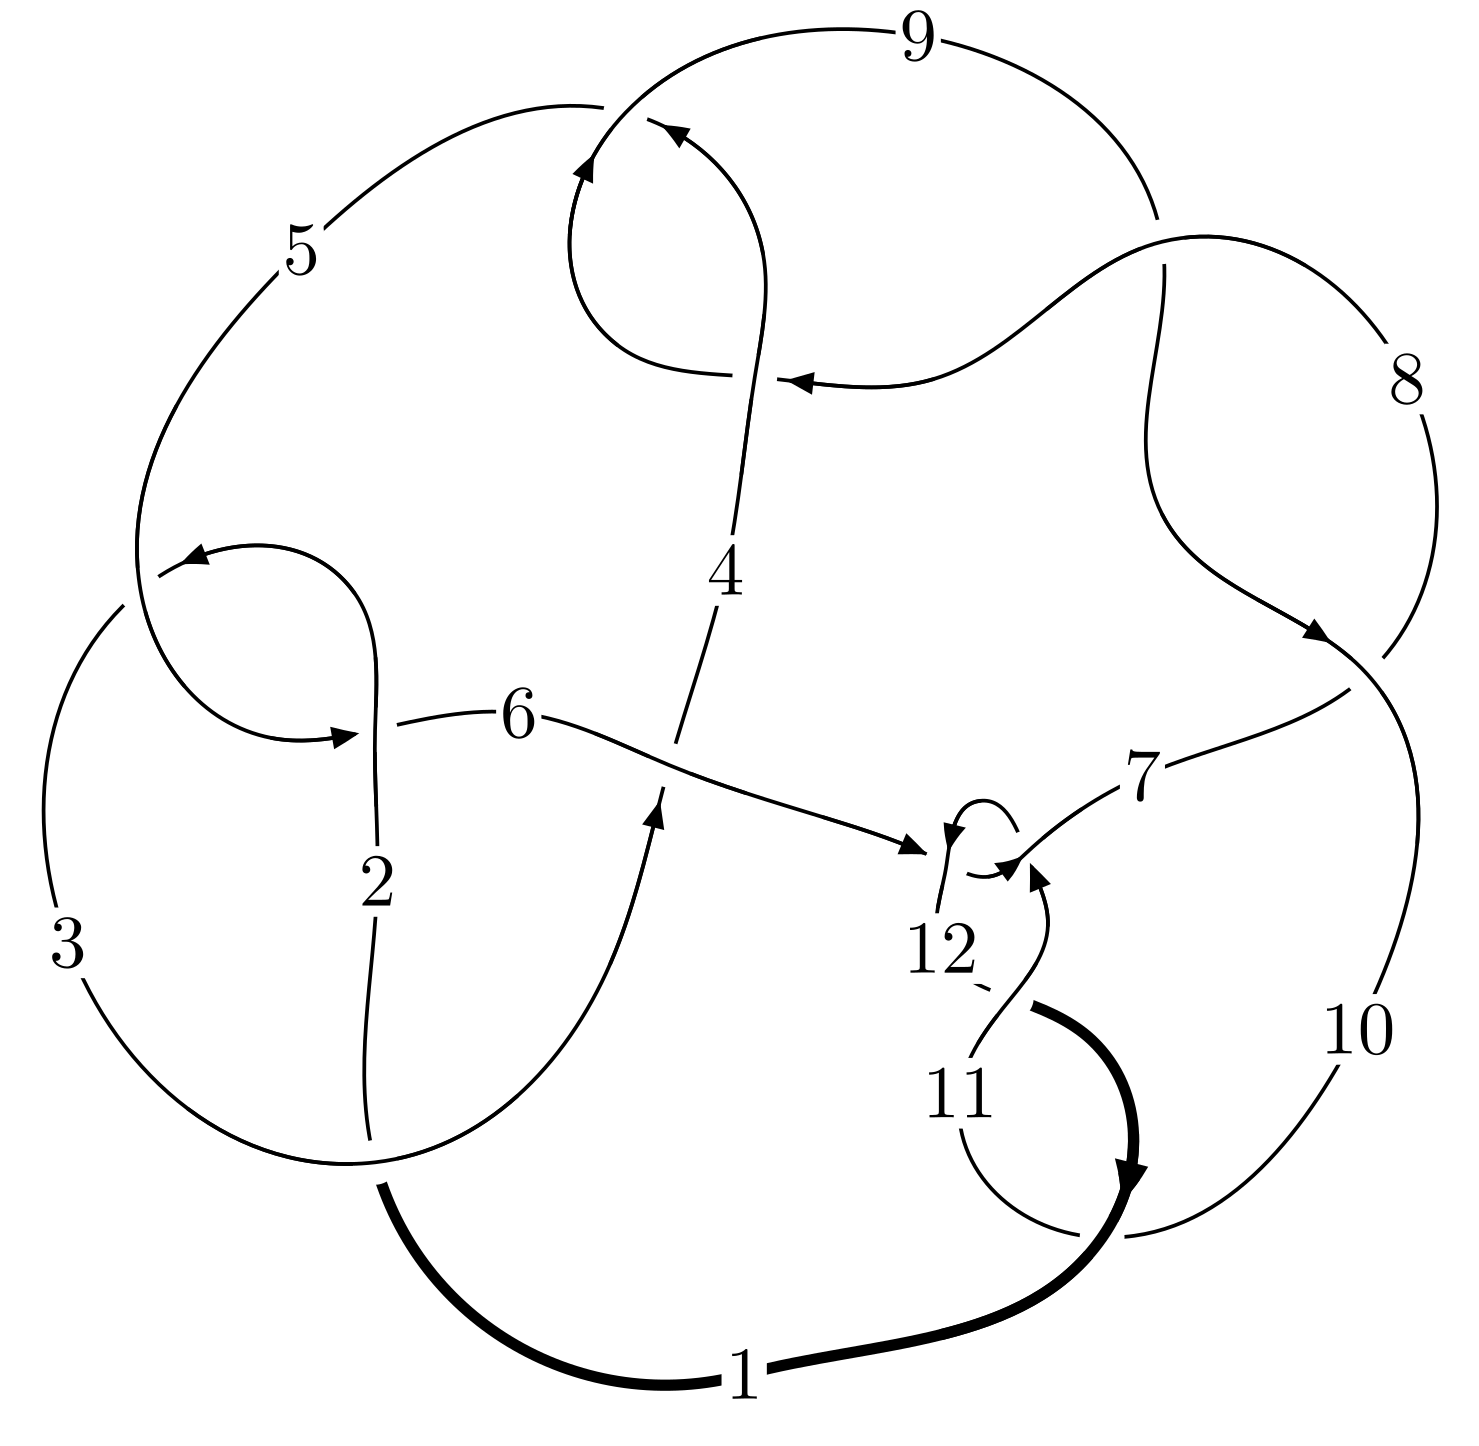
\includegraphics[width=112pt]{../../../GIT/diagram.site/Diagrams/png/829_12a_0028.png}\\
\ \ \ A knot diagram\footnotemark}&
\allowdisplaybreaks
\textbf{Linearized knot diagam} \\
\cline{2-2}
 &
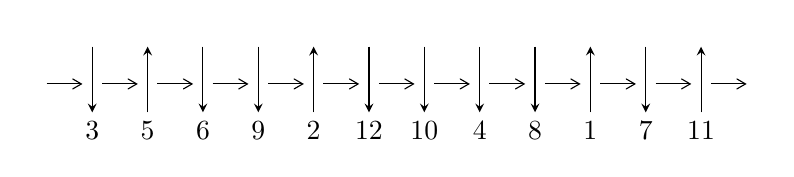
\begin{tikzpicture}[x=20pt, y=17pt]
	% nodes
	\node (C0) at (0, 0) {};
	\node (C1) at (1, 0) {};
	\node (C1U) at (1, +1) {};
	\node (C1D) at (1, -1) {3};

	\node (C2) at (2, 0) {};
	\node (C2U) at (2, +1) {};
	\node (C2D) at (2, -1) {5};

	\node (C3) at (3, 0) {};
	\node (C3U) at (3, +1) {};
	\node (C3D) at (3, -1) {6};

	\node (C4) at (4, 0) {};
	\node (C4U) at (4, +1) {};
	\node (C4D) at (4, -1) {9};

	\node (C5) at (5, 0) {};
	\node (C5U) at (5, +1) {};
	\node (C5D) at (5, -1) {2};

	\node (C6) at (6, 0) {};
	\node (C6U) at (6, +1) {};
	\node (C6D) at (6, -1) {12};

	\node (C7) at (7, 0) {};
	\node (C7U) at (7, +1) {};
	\node (C7D) at (7, -1) {10};

	\node (C8) at (8, 0) {};
	\node (C8U) at (8, +1) {};
	\node (C8D) at (8, -1) {4};

	\node (C9) at (9, 0) {};
	\node (C9U) at (9, +1) {};
	\node (C9D) at (9, -1) {8};

	\node (C10) at (10, 0) {};
	\node (C10U) at (10, +1) {};
	\node (C10D) at (10, -1) {1};

	\node (C11) at (11, 0) {};
	\node (C11U) at (11, +1) {};
	\node (C11D) at (11, -1) {7};

	\node (C12) at (12, 0) {};
	\node (C12U) at (12, +1) {};
	\node (C12D) at (12, -1) {11};
	\node (C13) at (13, 0) {};

	% arrows
	\draw[->,>={angle 60}]
	(C0) edge (C1) (C1) edge (C2) (C2) edge (C3) (C3) edge (C4) (C4) edge (C5) (C5) edge (C6) (C6) edge (C7) (C7) edge (C8) (C8) edge (C9) (C9) edge (C10) (C10) edge (C11) (C11) edge (C12) (C12) edge (C13) ;	\draw[->,>=stealth]
	(C1U) edge (C1D) (C2D) edge (C2U) (C3U) edge (C3D) (C4U) edge (C4D) (C5D) edge (C5U) (C6U) edge (C6D) (C7U) edge (C7D) (C8U) edge (C8D) (C9U) edge (C9D) (C10D) edge (C10U) (C11U) edge (C11D) (C12D) edge (C12U) ;
	\end{tikzpicture} \\
\hhline{~~} \\& 
\textbf{Solving Sequence} \\ \cline{2-2} 
 &
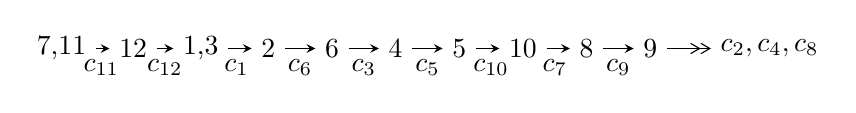
\begin{tikzpicture}[x=23pt, y=7pt]
	% node
	\node (A0) at (-1/8, 0) {7,11};
	\node (A1) at (1, 0) {12};
	\node (A2) at (33/16, 0) {1,3};
	\node (A3) at (25/8, 0) {2};
	\node (A4) at (33/8, 0) {6};
	\node (A5) at (41/8, 0) {4};
	\node (A6) at (49/8, 0) {5};
	\node (A7) at (57/8, 0) {10};
	\node (A8) at (65/8, 0) {8};
	\node (A9) at (73/8, 0) {9};
	\node (C1) at (1/2, -1) {$c_{11}$};
	\node (C2) at (3/2, -1) {$c_{12}$};
	\node (C3) at (21/8, -1) {$c_{1}$};
	\node (C4) at (29/8, -1) {$c_{6}$};
	\node (C5) at (37/8, -1) {$c_{3}$};
	\node (C6) at (45/8, -1) {$c_{5}$};
	\node (C7) at (53/8, -1) {$c_{10}$};
	\node (C8) at (61/8, -1) {$c_{7}$};
	\node (C9) at (69/8, -1) {$c_{9}$};
	\node (A10) at (11, 0) {$c_{2},c_{4},c_{8}$};

	% edge
	\draw[->,>=stealth]	
	(A0) edge (A1) (A1) edge (A2) (A2) edge (A3) (A3) edge (A4) (A4) edge (A5) (A5) edge (A6) (A6) edge (A7) (A7) edge (A8) (A8) edge (A9) ;
	\draw[->>,>={angle 60}]	
	(A9) edge (A10);
\end{tikzpicture} \\ 

\end{tabular} \\

\footnotetext{
The image of knot diagram is generated by the software ``\textbf{Draw programme}" developed by Andrew Bartholomew(\url{http://www.layer8.co.uk/maths/draw/index.htm\#Running-draw}), where we modified some parts for our purpose(\url{https://github.com/CATsTAILs/LinksPainter}).
}\phantom \\ \newline 
\centering \textbf{Ideals for irreducible components\footnotemark of $X_{\text{par}}$} 
 
\begin{align*}
I^u_{1}&=\langle 
u^{73}-2 u^{72}+\cdots+b-1,\;- u^{75}+3 u^{74}+\cdots+2 a-1,\;u^{76}-3 u^{75}+\cdots-4 u+1\rangle \\
I^u_{2}&=\langle 
b,\;a+u+1,\;u^2+u+1\rangle \\
I^u_{3}&=\langle 
b,\;a-1,\;u^{15}+3 u^{13}+6 u^{11}+u^{10}+7 u^9+2 u^8+6 u^7+3 u^6+5 u^5+2 u^4+3 u^3+u^2+2 u+1\rangle \\
I^u_{4}&=\langle 
b,\;a-1,\;u^2+u+1\rangle \\
\\
\end{align*}
\raggedright * 4 irreducible components of $\dim_{\mathbb{C}}=0$, with total 95 representations.\\
\footnotetext{All coefficients of polynomials are rational numbers. But the coefficients are sometimes approximated in decimal forms when there is not enough margin.}
\newpage
\renewcommand{\arraystretch}{1}
\centering \section*{I. $I^u_{1}= \langle u^{73}-2 u^{72}+\cdots+b-1,\;- u^{75}+3 u^{74}+\cdots+2 a-1,\;u^{76}-3 u^{75}+\cdots-4 u+1 \rangle$}
\flushleft \textbf{(i) Arc colorings}\\
\begin{tabular}{m{7pt} m{180pt} m{7pt} m{180pt} }
\flushright $a_{7}=$&$\begin{pmatrix}0\\u\end{pmatrix}$ \\
\flushright $a_{11}=$&$\begin{pmatrix}1\\0\end{pmatrix}$ \\
\flushright $a_{12}=$&$\begin{pmatrix}1\\u^2\end{pmatrix}$ \\
\flushright $a_{1}=$&$\begin{pmatrix}u^2+1\\u^2\end{pmatrix}$ \\
\flushright $a_{3}=$&$\begin{pmatrix}\frac{1}{2} u^{75}-\frac{3}{2} u^{74}+\cdots+4 u+\frac{1}{2}\\- u^{73}+2 u^{72}+\cdots-3 u+1\end{pmatrix}$ \\
\flushright $a_{2}=$&$\begin{pmatrix}-\frac{1}{2} u^{75}+\frac{3}{2} u^{74}+\cdots+2 u+\frac{5}{2}\\- u^{37}-7 u^{35}+\cdots-4 u^2- u\end{pmatrix}$ \\
\flushright $a_{6}=$&$\begin{pmatrix}u\\u^3+u\end{pmatrix}$ \\
\flushright $a_{4}=$&$\begin{pmatrix}u^{75}- u^{74}+\cdots+2 u+1\\3 u^{75}-\frac{11}{2} u^{74}+\cdots+\frac{5}{2} u-\frac{1}{2}\end{pmatrix}$ \\
\flushright $a_{5}=$&$\begin{pmatrix}- u^{75}+3 u^{74}+\cdots-8 u+1\\-\frac{1}{2} u^{74}+u^{73}+\cdots+\frac{5}{2} u-\frac{1}{2}\end{pmatrix}$ \\
\flushright $a_{10}=$&$\begin{pmatrix}u^4+u^2+1\\u^4\end{pmatrix}$ \\
\flushright $a_{8}=$&$\begin{pmatrix}- u^9-2 u^7-3 u^5-2 u^3- u\\- u^9- u^7- u^5+u\end{pmatrix}$ \\
\flushright $a_{9}=$&$\begin{pmatrix}u^{14}+3 u^{12}+6 u^{10}+7 u^8+6 u^6+4 u^4+2 u^2+1\\u^{14}+2 u^{12}+3 u^{10}+2 u^8- u^2\end{pmatrix}$\\&\end{tabular}
\flushleft \textbf{(ii) Obstruction class $= -1$}\\~\\
\flushleft \textbf{(iii) Cusp Shapes $= \frac{11}{2} u^{75}-19 u^{74}+\cdots+\frac{27}{2} u-7$}\\~\\
\newpage\renewcommand{\arraystretch}{1}
\flushleft \textbf{(iv) u-Polynomials at the component}\newline \\
\begin{tabular}{m{50pt}|m{274pt}}
Crossings & \hspace{64pt}u-Polynomials at each crossing \\
\hline $$\begin{aligned}c_{1}\end{aligned}$$&$\begin{aligned}
&u^{76}+35 u^{75}+\cdots-12 u^2+1
\end{aligned}$\\
\hline $$\begin{aligned}c_{2},c_{5}\end{aligned}$$&$\begin{aligned}
&u^{76}+3 u^{75}+\cdots+2 u+1
\end{aligned}$\\
\hline $$\begin{aligned}c_{3}\end{aligned}$$&$\begin{aligned}
&u^{76}-3 u^{75}+\cdots-2 u+1
\end{aligned}$\\
\hline $$\begin{aligned}c_{4},c_{8}\end{aligned}$$&$\begin{aligned}
&u^{76}+4 u^{75}+\cdots+16 u+16
\end{aligned}$\\
\hline $$\begin{aligned}c_{6},c_{11}\end{aligned}$$&$\begin{aligned}
&u^{76}-3 u^{75}+\cdots-4 u+1
\end{aligned}$\\
\hline $$\begin{aligned}c_{7},c_{9}\end{aligned}$$&$\begin{aligned}
&u^{76}+20 u^{75}+\cdots+1152 u+256
\end{aligned}$\\
\hline $$\begin{aligned}c_{10},c_{12}\end{aligned}$$&$\begin{aligned}
&u^{76}-27 u^{75}+\cdots+156 u^2+1
\end{aligned}$\\
\hline
\end{tabular}\\~\\
\newpage\renewcommand{\arraystretch}{1}
\flushleft \textbf{(v) Riley Polynomials at the component}\newline \\
\begin{tabular}{m{50pt}|m{274pt}}
Crossings & \hspace{64pt}Riley Polynomials at each crossing \\
\hline $$\begin{aligned}c_{1}\end{aligned}$$&$\begin{aligned}
&y^{76}+15 y^{75}+\cdots-24 y+1
\end{aligned}$\\
\hline $$\begin{aligned}c_{2},c_{5}\end{aligned}$$&$\begin{aligned}
&y^{76}+35 y^{75}+\cdots-12 y^2+1
\end{aligned}$\\
\hline $$\begin{aligned}c_{3}\end{aligned}$$&$\begin{aligned}
&y^{76}-5 y^{75}+\cdots-96 y+1
\end{aligned}$\\
\hline $$\begin{aligned}c_{4},c_{8}\end{aligned}$$&$\begin{aligned}
&y^{76}-20 y^{75}+\cdots-1152 y+256
\end{aligned}$\\
\hline $$\begin{aligned}c_{6},c_{11}\end{aligned}$$&$\begin{aligned}
&y^{76}+27 y^{75}+\cdots+156 y^2+1
\end{aligned}$\\
\hline $$\begin{aligned}c_{7},c_{9}\end{aligned}$$&$\begin{aligned}
&y^{76}+60 y^{75}+\cdots+712704 y+65536
\end{aligned}$\\
\hline $$\begin{aligned}c_{10},c_{12}\end{aligned}$$&$\begin{aligned}
&y^{76}+47 y^{75}+\cdots+312 y+1
\end{aligned}$\\
\hline
\end{tabular}\\~\\
\newpage\flushleft \textbf{(vi) Complex Volumes and Cusp Shapes}
$$\begin{array}{c|c|c}  
\text{Solutions to }I^u_{1}& \I (\text{vol} + \sqrt{-1}CS) & \text{Cusp shape}\\
 \hline 
\begin{aligned}
u &= \phantom{-}0.820067 + 0.580500 I \\
a &= -1.05528 - 2.33587 I \\
b &= \phantom{-}0.24200 - 2.52038 I\end{aligned}
 & \phantom{-}0.28459 + 11.09290 I & \phantom{-0.000000 } 0 \\ \hline\begin{aligned}
u &= \phantom{-}0.820067 - 0.580500 I \\
a &= -1.05528 + 2.33587 I \\
b &= \phantom{-}0.24200 + 2.52038 I\end{aligned}
 & \phantom{-}0.28459 - 11.09290 I & \phantom{-0.000000 } 0 \\ \hline\begin{aligned}
u &= \phantom{-}0.784162 + 0.610183 I \\
a &= \phantom{-}0.218261 - 1.162730 I \\
b &= \phantom{-}1.28826 - 0.84685 I\end{aligned}
 & -2.88911 + 3.62351 I & \phantom{-0.000000 } 0 \\ \hline\begin{aligned}
u &= \phantom{-}0.784162 - 0.610183 I \\
a &= \phantom{-}0.218261 + 1.162730 I \\
b &= \phantom{-}1.28826 + 0.84685 I\end{aligned}
 & -2.88911 - 3.62351 I & \phantom{-0.000000 } 0 \\ \hline\begin{aligned}
u &= \phantom{-}0.804404 + 0.574368 I \\
a &= \phantom{-}1.08811 + 1.63791 I \\
b &= -0.04056 + 1.69896 I\end{aligned}
 & \phantom{-}2.31596 + 5.81698 I & \phantom{-0.000000 } 0 \\ \hline\begin{aligned}
u &= \phantom{-}0.804404 - 0.574368 I \\
a &= \phantom{-}1.08811 - 1.63791 I \\
b &= -0.04056 - 1.69896 I\end{aligned}
 & \phantom{-}2.31596 - 5.81698 I & \phantom{-0.000000 } 0 \\ \hline\begin{aligned}
u &= -0.266450 + 1.003770 I \\
a &= -0.051209 - 0.894123 I \\
b &= \phantom{-}0.382872 + 0.726383 I\end{aligned}
 & -0.37911 + 6.19852 I & \phantom{-0.000000 } 0 \\ \hline\begin{aligned}
u &= -0.266450 - 1.003770 I \\
a &= -0.051209 + 0.894123 I \\
b &= \phantom{-}0.382872 - 0.726383 I\end{aligned}
 & -0.37911 - 6.19852 I & \phantom{-0.000000 } 0 \\ \hline\begin{aligned}
u &= -0.758972 + 0.572804 I \\
a &= -1.15206 + 2.58616 I \\
b &= \phantom{-}0.38835 + 2.61192 I\end{aligned}
 & \phantom{-}1.30562 - 4.85760 I & -4.00000 + 2.81637 I \\ \hline\begin{aligned}
u &= -0.758972 - 0.572804 I \\
a &= -1.15206 - 2.58616 I \\
b &= \phantom{-}0.38835 - 2.61192 I\end{aligned}
 & \phantom{-}1.30562 + 4.85760 I & -4.00000 - 2.81637 I\\
 \hline 
 \end{array}$$\newpage$$\begin{array}{c|c|c}  
\text{Solutions to }I^u_{1}& \I (\text{vol} + \sqrt{-1}CS) & \text{Cusp shape}\\
 \hline 
\begin{aligned}
u &= -0.614417 + 0.865433 I \\
a &= \phantom{-}0.80686 - 1.36588 I \\
b &= -0.59195 - 1.44117 I\end{aligned}
 & -0.59560 + 2.40827 I & \phantom{-0.000000 } 0 \\ \hline\begin{aligned}
u &= -0.614417 - 0.865433 I \\
a &= \phantom{-}0.80686 + 1.36588 I \\
b &= -0.59195 + 1.44117 I\end{aligned}
 & -0.59560 - 2.40827 I & \phantom{-0.000000 } 0 \\ \hline\begin{aligned}
u &= -0.682974 + 0.815558 I \\
a &= -2.87082 + 1.38786 I \\
b &= -0.95465 + 3.40719 I\end{aligned}
 & -3.11243 - 0.72332 I & \phantom{-0.000000 } 0 \\ \hline\begin{aligned}
u &= -0.682974 - 0.815558 I \\
a &= -2.87082 - 1.38786 I \\
b &= -0.95465 - 3.40719 I\end{aligned}
 & -3.11243 + 0.72332 I & \phantom{-0.000000 } 0 \\ \hline\begin{aligned}
u &= -0.215813 + 0.910718 I \\
a &= \phantom{-}0.265261 + 0.121375 I \\
b &= -0.586596 - 0.385311 I\end{aligned}
 & \phantom{-}1.49867 + 2.13083 I & \phantom{-0.000000 } 0. - 5.38892 I \\ \hline\begin{aligned}
u &= -0.215813 - 0.910718 I \\
a &= \phantom{-}0.265261 - 0.121375 I \\
b &= -0.586596 + 0.385311 I\end{aligned}
 & \phantom{-}1.49867 - 2.13083 I & \phantom{-0.000000 -}0. + 5.38892 I \\ \hline\begin{aligned}
u &= \phantom{-}0.737672 + 0.767805 I \\
a &= \phantom{-}1.05157 + 1.41551 I \\
b &= -0.22256 + 1.66158 I\end{aligned}
 & -4.16374 + 0.54928 I & \phantom{-0.000000 } 0 \\ \hline\begin{aligned}
u &= \phantom{-}0.737672 - 0.767805 I \\
a &= \phantom{-}1.05157 - 1.41551 I \\
b &= -0.22256 - 1.66158 I\end{aligned}
 & -4.16374 - 0.54928 I & \phantom{-0.000000 } 0 \\ \hline\begin{aligned}
u &= -0.744701 + 0.542472 I \\
a &= \phantom{-}1.18253 - 1.67888 I \\
b &= -0.01927 - 1.66588 I\end{aligned}
 & \phantom{-}3.09050 + 0.22669 I & -1.99230 - 2.08336 I \\ \hline\begin{aligned}
u &= -0.744701 - 0.542472 I \\
a &= \phantom{-}1.18253 + 1.67888 I \\
b &= -0.01927 + 1.66588 I\end{aligned}
 & \phantom{-}3.09050 - 0.22669 I & -1.99230 + 2.08336 I\\
 \hline 
 \end{array}$$\newpage$$\begin{array}{c|c|c}  
\text{Solutions to }I^u_{1}& \I (\text{vol} + \sqrt{-1}CS) & \text{Cusp shape}\\
 \hline 
\begin{aligned}
u &= \phantom{-}0.774528 + 0.755664 I \\
a &= -1.82547 - 1.78464 I \\
b &= -0.27849 - 2.85903 I\end{aligned}
 & -6.90483 + 4.88361 I & \phantom{-0.000000 } 0 \\ \hline\begin{aligned}
u &= \phantom{-}0.774528 - 0.755664 I \\
a &= -1.82547 + 1.78464 I \\
b &= -0.27849 + 2.85903 I\end{aligned}
 & -6.90483 - 4.88361 I & \phantom{-0.000000 } 0 \\ \hline\begin{aligned}
u &= -0.636867 + 0.654546 I \\
a &= \phantom{-}1.10871 + 1.19060 I \\
b &= \phantom{-}1.71940 + 0.17017 I\end{aligned}
 & -1.56601 + 1.58828 I & -7.89253 - 2.90076 I \\ \hline\begin{aligned}
u &= -0.636867 - 0.654546 I \\
a &= \phantom{-}1.10871 - 1.19060 I \\
b &= \phantom{-}1.71940 - 0.17017 I\end{aligned}
 & -1.56601 - 1.58828 I & -7.89253 + 2.90076 I \\ \hline\begin{aligned}
u &= \phantom{-}0.639841 + 0.879271 I \\
a &= -0.543599 + 0.737979 I \\
b &= -0.075619 + 0.338430 I\end{aligned}
 & -0.96997 - 4.97477 I & \phantom{-0.000000 } 0 \\ \hline\begin{aligned}
u &= \phantom{-}0.639841 - 0.879271 I \\
a &= -0.543599 - 0.737979 I \\
b &= -0.075619 - 0.338430 I\end{aligned}
 & -0.96997 + 4.97477 I & \phantom{-0.000000 } 0 \\ \hline\begin{aligned}
u &= \phantom{-}0.716966 + 0.538440 I \\
a &= -0.779361 + 0.668048 I \\
b &= \phantom{-}0.292228 + 0.497426 I\end{aligned}
 & \phantom{-}1.60658 - 2.39995 I & -4.54324 + 1.90730 I \\ \hline\begin{aligned}
u &= \phantom{-}0.716966 - 0.538440 I \\
a &= -0.779361 - 0.668048 I \\
b &= \phantom{-}0.292228 - 0.497426 I\end{aligned}
 & \phantom{-}1.60658 + 2.39995 I & -4.54324 - 1.90730 I \\ \hline\begin{aligned}
u &= -0.528629 + 0.969740 I \\
a &= -0.495625 - 0.870919 I \\
b &= -0.596905 + 0.163211 I\end{aligned}
 & -0.23592 + 3.03712 I & \phantom{-0.000000 } 0 \\ \hline\begin{aligned}
u &= -0.528629 - 0.969740 I \\
a &= -0.495625 + 0.870919 I \\
b &= -0.596905 - 0.163211 I\end{aligned}
 & -0.23592 - 3.03712 I & \phantom{-0.000000 } 0\\
 \hline 
 \end{array}$$\newpage$$\begin{array}{c|c|c}  
\text{Solutions to }I^u_{1}& \I (\text{vol} + \sqrt{-1}CS) & \text{Cusp shape}\\
 \hline 
\begin{aligned}
u &= \phantom{-}0.014582 + 1.106940 I \\
a &= \phantom{-}0.698613 + 0.845252 I \\
b &= \phantom{-}0.83233 - 1.27996 I\end{aligned}
 & \phantom{-}6.97493 - 3.72971 I & \phantom{-0.000000 } 0 \\ \hline\begin{aligned}
u &= \phantom{-}0.014582 - 1.106940 I \\
a &= \phantom{-}0.698613 - 0.845252 I \\
b &= \phantom{-}0.83233 + 1.27996 I\end{aligned}
 & \phantom{-}6.97493 + 3.72971 I & \phantom{-0.000000 } 0 \\ \hline\begin{aligned}
u &= \phantom{-}0.759065 + 0.810624 I \\
a &= -0.21510 - 2.16462 I \\
b &= \phantom{-}1.83924 - 1.72824 I\end{aligned}
 & -7.82704 - 2.79074 I & \phantom{-0.000000 } 0 \\ \hline\begin{aligned}
u &= \phantom{-}0.759065 - 0.810624 I \\
a &= -0.21510 + 2.16462 I \\
b &= \phantom{-}1.83924 + 1.72824 I\end{aligned}
 & -7.82704 + 2.79074 I & \phantom{-0.000000 } 0 \\ \hline\begin{aligned}
u &= -0.003461 + 1.114350 I \\
a &= -0.484952 - 0.498420 I \\
b &= -1.039760 + 0.702363 I\end{aligned}
 & \phantom{-}8.62942 + 1.55231 I & \phantom{-0.000000 } 0 \\ \hline\begin{aligned}
u &= -0.003461 - 1.114350 I \\
a &= -0.484952 + 0.498420 I \\
b &= -1.039760 - 0.702363 I\end{aligned}
 & \phantom{-}8.62942 - 1.55231 I & \phantom{-0.000000 } 0 \\ \hline\begin{aligned}
u &= -0.678647 + 0.889200 I \\
a &= -0.99601 + 3.18933 I \\
b &= \phantom{-}2.29317 + 2.94183 I\end{aligned}
 & -2.88720 + 5.97422 I & \phantom{-0.000000 } 0 \\ \hline\begin{aligned}
u &= -0.678647 - 0.889200 I \\
a &= -0.99601 - 3.18933 I \\
b &= \phantom{-}2.29317 - 2.94183 I\end{aligned}
 & -2.88720 - 5.97422 I & \phantom{-0.000000 } 0 \\ \hline\begin{aligned}
u &= -0.756171 + 0.426179 I \\
a &= -0.797372 - 0.584543 I \\
b &= \phantom{-}0.344833 - 0.560635 I\end{aligned}
 & \phantom{-}1.18722 + 7.92961 I & -5.68516 - 7.58189 I \\ \hline\begin{aligned}
u &= -0.756171 - 0.426179 I \\
a &= -0.797372 + 0.584543 I \\
b &= \phantom{-}0.344833 + 0.560635 I\end{aligned}
 & \phantom{-}1.18722 - 7.92961 I & -5.68516 + 7.58189 I\\
 \hline 
 \end{array}$$\newpage$$\begin{array}{c|c|c}  
\text{Solutions to }I^u_{1}& \I (\text{vol} + \sqrt{-1}CS) & \text{Cusp shape}\\
 \hline 
\begin{aligned}
u &= -0.040806 + 1.132090 I \\
a &= -0.446780 + 0.376335 I \\
b &= -0.941823 - 0.709155 I\end{aligned}
 & \phantom{-}8.37243 + 4.62112 I & \phantom{-0.000000 } 0 \\ \hline\begin{aligned}
u &= -0.040806 - 1.132090 I \\
a &= -0.446780 - 0.376335 I \\
b &= -0.941823 + 0.709155 I\end{aligned}
 & \phantom{-}8.37243 - 4.62112 I & \phantom{-0.000000 } 0 \\ \hline\begin{aligned}
u &= -0.054219 + 1.140020 I \\
a &= \phantom{-}0.589590 - 0.733142 I \\
b &= \phantom{-}0.70115 + 1.27546 I\end{aligned}
 & \phantom{-}6.50055 + 9.90761 I & \phantom{-0.000000 } 0 \\ \hline\begin{aligned}
u &= -0.054219 - 1.140020 I \\
a &= \phantom{-}0.589590 + 0.733142 I \\
b &= \phantom{-}0.70115 - 1.27546 I\end{aligned}
 & \phantom{-}6.50055 - 9.90761 I & \phantom{-0.000000 } 0 \\ \hline\begin{aligned}
u &= \phantom{-}0.735374 + 0.908373 I \\
a &= -1.93507 - 0.56007 I \\
b &= -1.05640 - 2.40281 I\end{aligned}
 & -7.52975 - 2.85954 I & \phantom{-0.000000 } 0 \\ \hline\begin{aligned}
u &= \phantom{-}0.735374 - 0.908373 I \\
a &= -1.93507 + 0.56007 I \\
b &= -1.05640 + 2.40281 I\end{aligned}
 & -7.52975 + 2.85954 I & \phantom{-0.000000 } 0 \\ \hline\begin{aligned}
u &= \phantom{-}0.707706 + 0.935010 I \\
a &= \phantom{-}1.03539 + 1.48069 I \\
b &= -0.48512 + 1.88720 I\end{aligned}
 & -3.65836 - 6.05326 I & \phantom{-0.000000 } 0 \\ \hline\begin{aligned}
u &= \phantom{-}0.707706 - 0.935010 I \\
a &= \phantom{-}1.03539 - 1.48069 I \\
b &= -0.48512 - 1.88720 I\end{aligned}
 & -3.65836 + 6.05326 I & \phantom{-0.000000 } 0 \\ \hline\begin{aligned}
u &= -0.632430 + 1.003530 I \\
a &= -1.272460 - 0.506257 I \\
b &= -1.24027 + 1.30625 I\end{aligned}
 & -0.49083 + 3.41773 I & \phantom{-0.000000 } 0 \\ \hline\begin{aligned}
u &= -0.632430 - 1.003530 I \\
a &= -1.272460 + 0.506257 I \\
b &= -1.24027 - 1.30625 I\end{aligned}
 & -0.49083 - 3.41773 I & \phantom{-0.000000 } 0\\
 \hline 
 \end{array}$$\newpage$$\begin{array}{c|c|c}  
\text{Solutions to }I^u_{1}& \I (\text{vol} + \sqrt{-1}CS) & \text{Cusp shape}\\
 \hline 
\begin{aligned}
u &= \phantom{-}0.727570 + 0.952707 I \\
a &= -1.41975 - 2.28891 I \\
b &= \phantom{-}1.28428 - 2.82954 I\end{aligned}
 & -6.30922 - 10.55470 I & \phantom{-0.000000 } 0 \\ \hline\begin{aligned}
u &= \phantom{-}0.727570 - 0.952707 I \\
a &= -1.41975 + 2.28891 I \\
b &= \phantom{-}1.28428 + 2.82954 I\end{aligned}
 & -6.30922 + 10.55470 I & \phantom{-0.000000 } 0 \\ \hline\begin{aligned}
u &= -0.014242 + 0.784224 I \\
a &= \phantom{-}0.639035 - 0.926041 I \\
b &= -0.869179 - 0.194601 I\end{aligned}
 & \phantom{-}2.08815 + 1.38840 I & \phantom{-}2.95491 - 3.97928 I \\ \hline\begin{aligned}
u &= -0.014242 - 0.784224 I \\
a &= \phantom{-}0.639035 + 0.926041 I \\
b &= -0.869179 + 0.194601 I\end{aligned}
 & \phantom{-}2.08815 - 1.38840 I & \phantom{-}2.95491 + 3.97928 I \\ \hline\begin{aligned}
u &= -0.619260 + 1.054980 I \\
a &= -0.429463 - 0.595270 I \\
b &= -0.312184 - 0.533722 I\end{aligned}
 & \phantom{-}4.72824 + 2.31494 I & \phantom{-0.000000 } 0 \\ \hline\begin{aligned}
u &= -0.619260 - 1.054980 I \\
a &= -0.429463 + 0.595270 I \\
b &= -0.312184 + 0.533722 I\end{aligned}
 & \phantom{-}4.72824 - 2.31494 I & \phantom{-0.000000 } 0 \\ \hline\begin{aligned}
u &= -0.650542 + 1.042030 I \\
a &= \phantom{-}1.34113 - 1.51578 I \\
b &= -0.49049 - 2.32412 I\end{aligned}
 & \phantom{-}4.53764 + 5.08932 I & \phantom{-0.000000 } 0 \\ \hline\begin{aligned}
u &= -0.650542 - 1.042030 I \\
a &= \phantom{-}1.34113 + 1.51578 I \\
b &= -0.49049 + 2.32412 I\end{aligned}
 & \phantom{-}4.53764 - 5.08932 I & \phantom{-0.000000 } 0 \\ \hline\begin{aligned}
u &= \phantom{-}0.655264 + 1.042540 I \\
a &= -0.467205 + 0.606561 I \\
b &= -0.260958 + 0.532361 I\end{aligned}
 & \phantom{-}4.45459 - 8.18431 I & \phantom{-0.000000 } 0 \\ \hline\begin{aligned}
u &= \phantom{-}0.655264 - 1.042540 I \\
a &= -0.467205 - 0.606561 I \\
b &= -0.260958 - 0.532361 I\end{aligned}
 & \phantom{-}4.45459 + 8.18431 I & \phantom{-0.000000 } 0\\
 \hline 
 \end{array}$$\newpage$$\begin{array}{c|c|c}  
\text{Solutions to }I^u_{1}& \I (\text{vol} + \sqrt{-1}CS) & \text{Cusp shape}\\
 \hline 
\begin{aligned}
u &= -0.663246 + 1.039230 I \\
a &= -2.27057 + 1.76444 I \\
b &= \phantom{-}0.36310 + 3.31027 I\end{aligned}
 & \phantom{-}2.67522 + 10.26500 I & \phantom{-0.000000 } 0 \\ \hline\begin{aligned}
u &= -0.663246 - 1.039230 I \\
a &= -2.27057 - 1.76444 I \\
b &= \phantom{-}0.36310 - 3.31027 I\end{aligned}
 & \phantom{-}2.67522 - 10.26500 I & \phantom{-0.000000 } 0 \\ \hline\begin{aligned}
u &= \phantom{-}0.681711 + 1.035000 I \\
a &= -1.189270 + 0.104639 I \\
b &= -0.94885 - 1.58563 I\end{aligned}
 & -1.62052 - 9.16663 I & \phantom{-0.000000 } 0 \\ \hline\begin{aligned}
u &= \phantom{-}0.681711 - 1.035000 I \\
a &= -1.189270 - 0.104639 I \\
b &= -0.94885 + 1.58563 I\end{aligned}
 & -1.62052 + 9.16663 I & \phantom{-0.000000 } 0 \\ \hline\begin{aligned}
u &= \phantom{-}0.677356 + 1.053730 I \\
a &= \phantom{-}1.29035 + 1.43391 I \\
b &= -0.40380 + 2.25686 I\end{aligned}
 & \phantom{-}3.74543 - 11.38940 I & \phantom{-0.000000 } 0 \\ \hline\begin{aligned}
u &= \phantom{-}0.677356 - 1.053730 I \\
a &= \phantom{-}1.29035 - 1.43391 I \\
b &= -0.40380 - 2.25686 I\end{aligned}
 & \phantom{-}3.74543 + 11.38940 I & \phantom{-0.000000 } 0 \\ \hline\begin{aligned}
u &= \phantom{-}0.684596 + 1.057450 I \\
a &= -2.07654 - 1.62476 I \\
b &= \phantom{-}0.33793 - 3.06189 I\end{aligned}
 & \phantom{-}1.7152 - 16.7334 I & \phantom{-0.000000 } 0 \\ \hline\begin{aligned}
u &= \phantom{-}0.684596 - 1.057450 I \\
a &= -2.07654 + 1.62476 I \\
b &= \phantom{-}0.33793 + 3.06189 I\end{aligned}
 & \phantom{-}1.7152 + 16.7334 I & \phantom{-0.000000 } 0 \\ \hline\begin{aligned}
u &= -0.607659 + 0.388530 I \\
a &= \phantom{-}0.330601 + 0.231355 I \\
b &= \phantom{-}0.754959 + 0.436898 I\end{aligned}
 & -1.72401 + 1.26068 I & -9.61689 - 3.20971 I \\ \hline\begin{aligned}
u &= -0.607659 - 0.388530 I \\
a &= \phantom{-}0.330601 - 0.231355 I \\
b &= \phantom{-}0.754959 - 0.436898 I\end{aligned}
 & -1.72401 - 1.26068 I & -9.61689 + 3.20971 I\\
 \hline 
 \end{array}$$\newpage$$\begin{array}{c|c|c}  
\text{Solutions to }I^u_{1}& \I (\text{vol} + \sqrt{-1}CS) & \text{Cusp shape}\\
 \hline 
\begin{aligned}
u &= \phantom{-}0.141223 + 0.694571 I \\
a &= -0.45492 + 1.73909 I \\
b &= \phantom{-}0.930270 - 0.034337 I\end{aligned}
 & \phantom{-}1.00182 - 2.99656 I & \phantom{-}0.34736 + 1.79586 I \\ \hline\begin{aligned}
u &= \phantom{-}0.141223 - 0.694571 I \\
a &= -0.45492 - 1.73909 I \\
b &= \phantom{-}0.930270 + 0.034337 I\end{aligned}
 & \phantom{-}1.00182 + 2.99656 I & \phantom{-}0.34736 - 1.79586 I \\ \hline\begin{aligned}
u &= -0.606989 + 0.079902 I \\
a &= -0.801617 - 0.099145 I \\
b &= \phantom{-}0.509633 - 0.600376 I\end{aligned}
 & -3.65273 + 3.42052 I & -12.40083 - 4.88890 I \\ \hline\begin{aligned}
u &= -0.606989 - 0.079902 I \\
a &= -0.801617 + 0.099145 I \\
b &= \phantom{-}0.509633 + 0.600376 I\end{aligned}
 & -3.65273 - 3.42052 I & -12.40083 + 4.88890 I \\ \hline\begin{aligned}
u &= \phantom{-}0.214408 + 0.135150 I \\
a &= \phantom{-}0.38448 + 2.43399 I \\
b &= \phantom{-}0.411442 - 0.639233 I\end{aligned}
 & -0.32678 + 1.73919 I & -2.49698 - 4.03216 I \\ \hline\begin{aligned}
u &= \phantom{-}0.214408 - 0.135150 I \\
a &= \phantom{-}0.38448 - 2.43399 I \\
b &= \phantom{-}0.411442 + 0.639233 I\end{aligned}
 & -0.32678 - 1.73919 I & -2.49698 + 4.03216 I\\
 \hline 
 \end{array}$$\newpage\newpage\renewcommand{\arraystretch}{1}
\centering \section*{II. $I^u_{2}= \langle b,\;a+u+1,\;u^2+u+1 \rangle$}
\flushleft \textbf{(i) Arc colorings}\\
\begin{tabular}{m{7pt} m{180pt} m{7pt} m{180pt} }
\flushright $a_{7}=$&$\begin{pmatrix}0\\u\end{pmatrix}$ \\
\flushright $a_{11}=$&$\begin{pmatrix}1\\0\end{pmatrix}$ \\
\flushright $a_{12}=$&$\begin{pmatrix}1\\- u-1\end{pmatrix}$ \\
\flushright $a_{1}=$&$\begin{pmatrix}- u\\- u-1\end{pmatrix}$ \\
\flushright $a_{3}=$&$\begin{pmatrix}- u-1\\0\end{pmatrix}$ \\
\flushright $a_{2}=$&$\begin{pmatrix}- u-1\\- u-1\end{pmatrix}$ \\
\flushright $a_{6}=$&$\begin{pmatrix}u\\u+1\end{pmatrix}$ \\
\flushright $a_{4}=$&$\begin{pmatrix}0\\1\end{pmatrix}$ \\
\flushright $a_{5}=$&$\begin{pmatrix}0\\1\end{pmatrix}$ \\
\flushright $a_{10}=$&$\begin{pmatrix}0\\u\end{pmatrix}$ \\
\flushright $a_{8}=$&$\begin{pmatrix}0\\u\end{pmatrix}$ \\
\flushright $a_{9}=$&$\begin{pmatrix}0\\u\end{pmatrix}$\\&\end{tabular}
\flushleft \textbf{(ii) Obstruction class $= 1$}\\~\\
\flushleft \textbf{(iii) Cusp Shapes $= -8 u-7$}\\~\\
\newpage\renewcommand{\arraystretch}{1}
\flushleft \textbf{(iv) u-Polynomials at the component}\newline \\
\begin{tabular}{m{50pt}|m{274pt}}
Crossings & \hspace{64pt}u-Polynomials at each crossing \\
\hline $$\begin{aligned}c_{1},c_{3},c_{5}\\c_{6},c_{12}\end{aligned}$$&$\begin{aligned}
&u^2- u+1
\end{aligned}$\\
\hline $$\begin{aligned}c_{2},c_{10},c_{11}\end{aligned}$$&$\begin{aligned}
&u^2+u+1
\end{aligned}$\\
\hline $$\begin{aligned}c_{4},c_{7},c_{8}\\c_{9}\end{aligned}$$&$\begin{aligned}
&u^2
\end{aligned}$\\
\hline
\end{tabular}\\~\\
\newpage\renewcommand{\arraystretch}{1}
\flushleft \textbf{(v) Riley Polynomials at the component}\newline \\
\begin{tabular}{m{50pt}|m{274pt}}
Crossings & \hspace{64pt}Riley Polynomials at each crossing \\
\hline $$\begin{aligned}c_{1},c_{2},c_{3}\\c_{5},c_{6},c_{10}\\c_{11},c_{12}\end{aligned}$$&$\begin{aligned}
&y^2+y+1
\end{aligned}$\\
\hline $$\begin{aligned}c_{4},c_{7},c_{8}\\c_{9}\end{aligned}$$&$\begin{aligned}
&y^2
\end{aligned}$\\
\hline
\end{tabular}\\~\\
\newpage\flushleft \textbf{(vi) Complex Volumes and Cusp Shapes}
$$\begin{array}{c|c|c}  
\text{Solutions to }I^u_{2}& \I (\text{vol} + \sqrt{-1}CS) & \text{Cusp shape}\\
 \hline 
\begin{aligned}
u &= -0.500000 + 0.866025 I \\
a &= -0.500000 - 0.866025 I \\
b &= \phantom{-0.000000 } 0\end{aligned}
 & \phantom{-0.000000 -}4.05977 I & -3.00000 - 6.92820 I \\ \hline\begin{aligned}
u &= -0.500000 - 0.866025 I \\
a &= -0.500000 + 0.866025 I \\
b &= \phantom{-0.000000 } 0\end{aligned}
 & \phantom{-0.000000 } -4.05977 I & -3.00000 + 6.92820 I\\
 \hline 
 \end{array}$$\newpage\newpage\renewcommand{\arraystretch}{1}
\centering \section*{III. $I^u_{3}= \langle b,\;a-1,\;u^{15}+3 u^{13}+\cdots+2 u+1 \rangle$}
\flushleft \textbf{(i) Arc colorings}\\
\begin{tabular}{m{7pt} m{180pt} m{7pt} m{180pt} }
\flushright $a_{7}=$&$\begin{pmatrix}0\\u\end{pmatrix}$ \\
\flushright $a_{11}=$&$\begin{pmatrix}1\\0\end{pmatrix}$ \\
\flushright $a_{12}=$&$\begin{pmatrix}1\\u^2\end{pmatrix}$ \\
\flushright $a_{1}=$&$\begin{pmatrix}u^2+1\\u^2\end{pmatrix}$ \\
\flushright $a_{3}=$&$\begin{pmatrix}1\\0\end{pmatrix}$ \\
\flushright $a_{2}=$&$\begin{pmatrix}1\\u^2\end{pmatrix}$ \\
\flushright $a_{6}=$&$\begin{pmatrix}u\\u^3+u\end{pmatrix}$ \\
\flushright $a_{4}=$&$\begin{pmatrix}u^4+u^2+1\\u^6+2 u^4+u^2\end{pmatrix}$ \\
\flushright $a_{5}=$&$\begin{pmatrix}0\\u\end{pmatrix}$ \\
\flushright $a_{10}=$&$\begin{pmatrix}u^4+u^2+1\\u^4\end{pmatrix}$ \\
\flushright $a_{8}=$&$\begin{pmatrix}- u^9-2 u^7-3 u^5-2 u^3- u\\- u^9- u^7- u^5+u\end{pmatrix}$ \\
\flushright $a_{9}=$&$\begin{pmatrix}u^{14}+3 u^{12}+6 u^{10}+7 u^8+6 u^6+4 u^4+2 u^2+1\\u^{14}+2 u^{12}+3 u^{10}+2 u^8- u^2\end{pmatrix}$\\&\end{tabular}
\flushleft \textbf{(ii) Obstruction class $= -1$}\\~\\
\flushleft \textbf{(iii) Cusp Shapes $= -4 u^{10}-8 u^8-12 u^6-4 u^5-8 u^4-4 u^3-4 u^2-4 u-10$}\\~\\
\newpage\renewcommand{\arraystretch}{1}
\flushleft \textbf{(iv) u-Polynomials at the component}\newline \\
\begin{tabular}{m{50pt}|m{274pt}}
Crossings & \hspace{64pt}u-Polynomials at each crossing \\
\hline $$\begin{aligned}c_{1}\end{aligned}$$&$\begin{aligned}
&u^{15}+6 u^{14}+\cdots+2 u-1
\end{aligned}$\\
\hline $$\begin{aligned}c_{2},c_{5},c_{6}\\c_{11}\end{aligned}$$&$\begin{aligned}
&u^{15}+3 u^{13}+\cdots+2 u+1
\end{aligned}$\\
\hline $$\begin{aligned}c_{3}\end{aligned}$$&$\begin{aligned}
&u^{15}+3 u^{13}+\cdots-4 u+1
\end{aligned}$\\
\hline $$\begin{aligned}c_{4},c_{8}\end{aligned}$$&$\begin{aligned}
&(u^3- u^2+1)^5
\end{aligned}$\\
\hline $$\begin{aligned}c_{7},c_{9}\end{aligned}$$&$\begin{aligned}
&(u^3+u^2+2 u+1)^5
\end{aligned}$\\
\hline $$\begin{aligned}c_{10},c_{12}\end{aligned}$$&$\begin{aligned}
&u^{15}-6 u^{14}+\cdots+2 u+1
\end{aligned}$\\
\hline
\end{tabular}\\~\\
\newpage\renewcommand{\arraystretch}{1}
\flushleft \textbf{(v) Riley Polynomials at the component}\newline \\
\begin{tabular}{m{50pt}|m{274pt}}
Crossings & \hspace{64pt}Riley Polynomials at each crossing \\
\hline $$\begin{aligned}c_{1},c_{10},c_{12}\end{aligned}$$&$\begin{aligned}
&y^{15}+6 y^{14}+\cdots+18 y-1
\end{aligned}$\\
\hline $$\begin{aligned}c_{2},c_{5},c_{6}\\c_{11}\end{aligned}$$&$\begin{aligned}
&y^{15}+6 y^{14}+\cdots+2 y-1
\end{aligned}$\\
\hline $$\begin{aligned}c_{3}\end{aligned}$$&$\begin{aligned}
&y^{15}+6 y^{14}+\cdots-14 y-1
\end{aligned}$\\
\hline $$\begin{aligned}c_{4},c_{8}\end{aligned}$$&$\begin{aligned}
&(y^3- y^2+2 y-1)^5
\end{aligned}$\\
\hline $$\begin{aligned}c_{7},c_{9}\end{aligned}$$&$\begin{aligned}
&(y^3+3 y^2+2 y-1)^5
\end{aligned}$\\
\hline
\end{tabular}\\~\\
\newpage\flushleft \textbf{(vi) Complex Volumes and Cusp Shapes}
$$\begin{array}{c|c|c}  
\text{Solutions to }I^u_{3}& \I (\text{vol} + \sqrt{-1}CS) & \text{Cusp shape}\\
 \hline 
\begin{aligned}
u &= \phantom{-}0.633840 + 0.835010 I \\
a &= \phantom{-}1.00000\phantom{ +0.000000I} \\
b &= \phantom{-0.000000 } 0\end{aligned}
 & -1.11345\phantom{ +0.000000I} & -9.01951 + 0. I\phantom{ +0.000000I} \\ \hline\begin{aligned}
u &= \phantom{-}0.633840 - 0.835010 I \\
a &= \phantom{-}1.00000\phantom{ +0.000000I} \\
b &= \phantom{-0.000000 } 0\end{aligned}
 & -1.11345\phantom{ +0.000000I} & -9.01951 + 0. I\phantom{ +0.000000I} \\ \hline\begin{aligned}
u &= -0.406029 + 0.986492 I \\
a &= \phantom{-}1.00000\phantom{ +0.000000I} \\
b &= \phantom{-0.000000 } 0\end{aligned}
 & -1.11345\phantom{ +0.000000I} & -9.01951 + 0. I\phantom{ +0.000000I} \\ \hline\begin{aligned}
u &= -0.406029 - 0.986492 I \\
a &= \phantom{-}1.00000\phantom{ +0.000000I} \\
b &= \phantom{-0.000000 } 0\end{aligned}
 & -1.11345\phantom{ +0.000000I} & -9.01951 + 0. I\phantom{ +0.000000I} \\ \hline\begin{aligned}
u &= \phantom{-}0.752750 + 0.551515 I \\
a &= \phantom{-}1.00000\phantom{ +0.000000I} \\
b &= \phantom{-0.000000 } 0\end{aligned}
 & \phantom{-}3.02413 + 2.82812 I & -2.49024 - 2.97945 I \\ \hline\begin{aligned}
u &= \phantom{-}0.752750 - 0.551515 I \\
a &= \phantom{-}1.00000\phantom{ +0.000000I} \\
b &= \phantom{-0.000000 } 0\end{aligned}
 & \phantom{-}3.02413 - 2.82812 I & -2.49024 + 2.97945 I \\ \hline\begin{aligned}
u &= -0.048319 + 1.089120 I \\
a &= \phantom{-}1.00000\phantom{ +0.000000I} \\
b &= \phantom{-0.000000 } 0\end{aligned}
 & \phantom{-}3.02413 + 2.82812 I & -2.49024 - 2.97945 I \\ \hline\begin{aligned}
u &= -0.048319 - 1.089120 I \\
a &= \phantom{-}1.00000\phantom{ +0.000000I} \\
b &= \phantom{-0.000000 } 0\end{aligned}
 & \phantom{-}3.02413 - 2.82812 I & -2.49024 + 2.97945 I \\ \hline\begin{aligned}
u &= -0.742775 + 0.457992 I \\
a &= \phantom{-}1.00000\phantom{ +0.000000I} \\
b &= \phantom{-0.000000 } 0\end{aligned}
 & \phantom{-}3.02413 + 2.82812 I & -2.49024 - 2.97945 I \\ \hline\begin{aligned}
u &= -0.742775 - 0.457992 I \\
a &= \phantom{-}1.00000\phantom{ +0.000000I} \\
b &= \phantom{-0.000000 } 0\end{aligned}
 & \phantom{-}3.02413 - 2.82812 I & -2.49024 + 2.97945 I\\
 \hline 
 \end{array}$$\newpage$$\begin{array}{c|c|c}  
\text{Solutions to }I^u_{3}& \I (\text{vol} + \sqrt{-1}CS) & \text{Cusp shape}\\
 \hline 
\begin{aligned}
u &= \phantom{-}0.644158 + 1.035000 I \\
a &= \phantom{-}1.00000\phantom{ +0.000000I} \\
b &= \phantom{-0.000000 } 0\end{aligned}
 & \phantom{-}3.02413 - 2.82812 I & -2.49024 + 2.97945 I \\ \hline\begin{aligned}
u &= \phantom{-}0.644158 - 1.035000 I \\
a &= \phantom{-}1.00000\phantom{ +0.000000I} \\
b &= \phantom{-0.000000 } 0\end{aligned}
 & \phantom{-}3.02413 + 2.82812 I & -2.49024 - 2.97945 I \\ \hline\begin{aligned}
u &= -0.605814 + 1.063630 I \\
a &= \phantom{-}1.00000\phantom{ +0.000000I} \\
b &= \phantom{-0.000000 } 0\end{aligned}
 & \phantom{-}3.02413 - 2.82812 I & -2.49024 + 2.97945 I \\ \hline\begin{aligned}
u &= -0.605814 - 1.063630 I \\
a &= \phantom{-}1.00000\phantom{ +0.000000I} \\
b &= \phantom{-0.000000 } 0\end{aligned}
 & \phantom{-}3.02413 + 2.82812 I & -2.49024 - 2.97945 I \\ \hline\begin{aligned}
u &= -0.455622\phantom{ +0.000000I} \\
a &= \phantom{-}1.00000\phantom{ +0.000000I} \\
b &= \phantom{-0.000000 } 0\end{aligned}
 & -1.11345\phantom{ +0.000000I} & -9.01950\phantom{ +0.000000I}\\
 \hline 
 \end{array}$$\newpage\newpage\renewcommand{\arraystretch}{1}
\centering \section*{IV. $I^u_{4}= \langle b,\;a-1,\;u^2+u+1 \rangle$}
\flushleft \textbf{(i) Arc colorings}\\
\begin{tabular}{m{7pt} m{180pt} m{7pt} m{180pt} }
\flushright $a_{7}=$&$\begin{pmatrix}0\\u\end{pmatrix}$ \\
\flushright $a_{11}=$&$\begin{pmatrix}1\\0\end{pmatrix}$ \\
\flushright $a_{12}=$&$\begin{pmatrix}1\\- u-1\end{pmatrix}$ \\
\flushright $a_{1}=$&$\begin{pmatrix}- u\\- u-1\end{pmatrix}$ \\
\flushright $a_{3}=$&$\begin{pmatrix}1\\0\end{pmatrix}$ \\
\flushright $a_{2}=$&$\begin{pmatrix}1\\- u-1\end{pmatrix}$ \\
\flushright $a_{6}=$&$\begin{pmatrix}u\\u+1\end{pmatrix}$ \\
\flushright $a_{4}=$&$\begin{pmatrix}0\\u\end{pmatrix}$ \\
\flushright $a_{5}=$&$\begin{pmatrix}0\\u\end{pmatrix}$ \\
\flushright $a_{10}=$&$\begin{pmatrix}0\\u\end{pmatrix}$ \\
\flushright $a_{8}=$&$\begin{pmatrix}0\\u\end{pmatrix}$ \\
\flushright $a_{9}=$&$\begin{pmatrix}0\\u\end{pmatrix}$\\&\end{tabular}
\flushleft \textbf{(ii) Obstruction class $= 1$}\\~\\
\flushleft \textbf{(iii) Cusp Shapes $= 0$}\\~\\
\newpage\renewcommand{\arraystretch}{1}
\flushleft \textbf{(iv) u-Polynomials at the component}\newline \\
\begin{tabular}{m{50pt}|m{274pt}}
Crossings & \hspace{64pt}u-Polynomials at each crossing \\
\hline $$\begin{aligned}c_{1},c_{3},c_{5}\\c_{6},c_{12}\end{aligned}$$&$\begin{aligned}
&u^2- u+1
\end{aligned}$\\
\hline $$\begin{aligned}c_{2},c_{10},c_{11}\end{aligned}$$&$\begin{aligned}
&u^2+u+1
\end{aligned}$\\
\hline $$\begin{aligned}c_{4},c_{7},c_{8}\\c_{9}\end{aligned}$$&$\begin{aligned}
&u^2
\end{aligned}$\\
\hline
\end{tabular}\\~\\
\newpage\renewcommand{\arraystretch}{1}
\flushleft \textbf{(v) Riley Polynomials at the component}\newline \\
\begin{tabular}{m{50pt}|m{274pt}}
Crossings & \hspace{64pt}Riley Polynomials at each crossing \\
\hline $$\begin{aligned}c_{1},c_{2},c_{3}\\c_{5},c_{6},c_{10}\\c_{11},c_{12}\end{aligned}$$&$\begin{aligned}
&y^2+y+1
\end{aligned}$\\
\hline $$\begin{aligned}c_{4},c_{7},c_{8}\\c_{9}\end{aligned}$$&$\begin{aligned}
&y^2
\end{aligned}$\\
\hline
\end{tabular}\\~\\
\newpage\flushleft \textbf{(vi) Complex Volumes and Cusp Shapes}
$$\begin{array}{c|c|c}  
\text{Solutions to }I^u_{4}& \I (\text{vol} + \sqrt{-1}CS) & \text{Cusp shape}\\
 \hline 
\begin{aligned}
u &= -0.500000 + 0.866025 I \\
a &= \phantom{-}1.00000\phantom{ +0.000000I} \\
b &= \phantom{-0.000000 } 0\end{aligned}
 & \phantom{-0.000000 } 0 & \phantom{-0.000000 } 0 \\ \hline\begin{aligned}
u &= -0.500000 - 0.866025 I \\
a &= \phantom{-}1.00000\phantom{ +0.000000I} \\
b &= \phantom{-0.000000 } 0\end{aligned}
 & \phantom{-0.000000 } 0 & \phantom{-0.000000 } 0\\
 \hline 
 \end{array}$$\newpage
\newpage\renewcommand{\arraystretch}{1}
\centering \section*{ V. u-Polynomials}
\begin{tabular}{m{50pt}|m{274pt}}
Crossings & \hspace{64pt}u-Polynomials at each crossing \\
\hline $$\begin{aligned}c_{1}\end{aligned}$$&$\begin{aligned}
&((u^2- u+1)^2)(u^{15}+6 u^{14}+\cdots+2 u-1)(u^{76}+35 u^{75}+\cdots-12 u^2+1)
\end{aligned}$\\
\hline $$\begin{aligned}c_{2}\end{aligned}$$&$\begin{aligned}
&((u^2+u+1)^2)(u^{15}+3 u^{13}+\cdots+2 u+1)(u^{76}+3 u^{75}+\cdots+2 u+1)
\end{aligned}$\\
\hline $$\begin{aligned}c_{3}\end{aligned}$$&$\begin{aligned}
&((u^2- u+1)^2)(u^{15}+3 u^{13}+\cdots-4 u+1)(u^{76}-3 u^{75}+\cdots-2 u+1)
\end{aligned}$\\
\hline $$\begin{aligned}c_{4},c_{8}\end{aligned}$$&$\begin{aligned}
&u^4(u^3- u^2+1)^5(u^{76}+4 u^{75}+\cdots+16 u+16)
\end{aligned}$\\
\hline $$\begin{aligned}c_{5}\end{aligned}$$&$\begin{aligned}
&((u^2- u+1)^2)(u^{15}+3 u^{13}+\cdots+2 u+1)(u^{76}+3 u^{75}+\cdots+2 u+1)
\end{aligned}$\\
\hline $$\begin{aligned}c_{6}\end{aligned}$$&$\begin{aligned}
&((u^2- u+1)^2)(u^{15}+3 u^{13}+\cdots+2 u+1)(u^{76}-3 u^{75}+\cdots-4 u+1)
\end{aligned}$\\
\hline $$\begin{aligned}c_{7},c_{9}\end{aligned}$$&$\begin{aligned}
&u^4(u^3+u^2+2 u+1)^5(u^{76}+20 u^{75}+\cdots+1152 u+256)
\end{aligned}$\\
\hline $$\begin{aligned}c_{10}\end{aligned}$$&$\begin{aligned}
&((u^2+u+1)^2)(u^{15}-6 u^{14}+\cdots+2 u+1)(u^{76}-27 u^{75}+\cdots+156 u^{2}+1)
\end{aligned}$\\
\hline $$\begin{aligned}c_{11}\end{aligned}$$&$\begin{aligned}
&((u^2+u+1)^2)(u^{15}+3 u^{13}+\cdots+2 u+1)(u^{76}-3 u^{75}+\cdots-4 u+1)
\end{aligned}$\\
\hline $$\begin{aligned}c_{12}\end{aligned}$$&$\begin{aligned}
&((u^2- u+1)^2)(u^{15}-6 u^{14}+\cdots+2 u+1)(u^{76}-27 u^{75}+\cdots+156 u^{2}+1)
\end{aligned}$\\
\hline
\end{tabular}\newpage\renewcommand{\arraystretch}{1}
\centering \section*{ VI. Riley Polynomials}
\begin{tabular}{m{50pt}|m{274pt}}
Crossings & \hspace{64pt}Riley Polynomials at each crossing \\
\hline $$\begin{aligned}c_{1}\end{aligned}$$&$\begin{aligned}
&((y^2+y+1)^2)(y^{15}+6 y^{14}+\cdots+18 y-1)(y^{76}+15 y^{75}+\cdots-24 y+1)
\end{aligned}$\\
\hline $$\begin{aligned}c_{2},c_{5}\end{aligned}$$&$\begin{aligned}
&((y^2+y+1)^2)(y^{15}+6 y^{14}+\cdots+2 y-1)(y^{76}+35 y^{75}+\cdots-12 y^2+1)
\end{aligned}$\\
\hline $$\begin{aligned}c_{3}\end{aligned}$$&$\begin{aligned}
&((y^2+y+1)^2)(y^{15}+6 y^{14}+\cdots-14 y-1)(y^{76}-5 y^{75}+\cdots-96 y+1)
\end{aligned}$\\
\hline $$\begin{aligned}c_{4},c_{8}\end{aligned}$$&$\begin{aligned}
&y^4(y^3- y^2+2 y-1)^5(y^{76}-20 y^{75}+\cdots-1152 y+256)
\end{aligned}$\\
\hline $$\begin{aligned}c_{6},c_{11}\end{aligned}$$&$\begin{aligned}
&((y^2+y+1)^2)(y^{15}+6 y^{14}+\cdots+2 y-1)(y^{76}+27 y^{75}+\cdots+156 y^{2}+1)
\end{aligned}$\\
\hline $$\begin{aligned}c_{7},c_{9}\end{aligned}$$&$\begin{aligned}
&y^4(y^3+3 y^2+2 y-1)^5(y^{76}+60 y^{75}+\cdots+712704 y+65536)
\end{aligned}$\\
\hline $$\begin{aligned}c_{10},c_{12}\end{aligned}$$&$\begin{aligned}
&((y^2+y+1)^2)(y^{15}+6 y^{14}+\cdots+18 y-1)\\
&\cdot(y^{76}+47 y^{75}+\cdots+312 y+1)
\end{aligned}$\\
\hline
\end{tabular}
\vskip 2pc
\end{document}